\input{preamble.tex}
\newcommand{\C}{\mathcal{C}}
\usepackage{makecell} % commande \thead, dans l'exo 1

\begin{document}
\pagestyle{fancy}
\fancyhead[L]{Seconde}
\fancyhead[C]{\textbf{DS n°5 — fonction carré, racine carrée, valeur absolue}}
\fancyhead[R]{\today}

\reversemarginpar

\null\vspace{-30pt}
Nom / Prénom : \\

Consignes particulières : 
\begin{itemize}[label=$\bullet$]
	\item 
	La calculatrice est \textbf{interdite}.
	\item 
	L'exercice \ref{exe:1} peut être fait entièrement sur la feuille d'évaluation. Écrire son nom avant de rendre le sujet pour qu'il soit corrigé.
	\item 
	Toute trace de recherche est prise en compte.
	%\item 
	%L'abbréviation $\tq$ signifie ``tel que''.
\end{itemize}

\hrule

\exe{2}{
	Vrai ou faux ? Cocher la case correspondante (aucune justification n'est attendue). \\
	\vspace{-20pt}
	\begin{center}
	\begin{tabular}{c c c}
		\hspace{10cm} & Vrai & Faux \\
		La fonction racine carrée est paire & \resizebox{10pt}{!}{$\square$} & \resizebox{10pt}{!}{$\square$}   \\
		 Pour $a, b \in \R$, si $a \leq b$ alors $a^2 \leq b^2$ & \resizebox{10pt}{!}{$\square$} & \resizebox{10pt}{!}{$\square$}   \\
	\end{tabular}
	\end{center}
}{exe:1}{
Les réponses sont, dans l'ordre : faux et faux.
}

\exe{4}{
Calculer

	\begin{multicols}{2}
	\begin{enumerate}[label=(\alph*)]
		\item $35^2 - 33^2$
		\item $95^2$ 
		\item $\sqrt{1,21}$
		\item $\sqrt{81~000~000}$
	\end{enumerate}
	\end{multicols}
	
}{exe:2}{
\begin{enumerate}[label=(\alph*)]
\item $35^2 - 33^2 = (35+33)(35-33) = 136$ ;
\item $95^2 = (100-5)^2 = 10~000 -2\times100\times5 + 25 = 9025$ ;
\item $\sqrt{1,21} = \dfrac{\sqrt{121}}{\sqrt{100}} = 1,1$ ;
\item  $\sqrt{81~000~000} = \sqrt{80} \times \sqrt{1~000~000} = 9~000$.
\end{enumerate}
}

\exe{4}{
	Écrire les nombres suivants sous la forme $a\sqrt{b}$ où $a\in\N$ est entier et $b\in\N$ est le 
	\textbf{plus petit entier naturel possible}.

	\begin{multicols}{2}
	\begin{enumerate}
		\item $\sqrt{20}$
		\item $2\sqrt{75}$
		\item $\dfrac{21}{\sqrt{7}}$
		\item $\sqrt{180}$
	\end{enumerate}
	\end{multicols}
}{exe:3}{
\begin{enumerate}[label=(\alph*)]
\item $\sqrt{20} = 2\sqrt{5}$
\item $2\sqrt{75} = 10\sqrt{3}$
\item $\dfrac{21}{\sqrt{7}} = 3 \sqrt{7}$
\item $\sqrt{180} = 6 \sqrt{5}$
\end{enumerate}
}

\exe{3}{
Pour chacun des cas ci-dessous, donner les valeurs possibles de $x$. Utiliser des intervalles si cela est pertinent.
	\begin{multicols}{2}
	\begin{enumerate}
		\item $\abs{2x-23} = 7$
		\item $\abs{x+3} \geq 12$
		\item $\abs{2x - 1} < 7$  
	\end{enumerate}
	\end{multicols}
}{exe:4}{
\begin{enumerate}
\item $x = 15$ et $x=8$ ;
\item $x \in ]-\infty ; -15 ]$ ou $x \in [9 ; + \infty [$ ;
\item $x \in ] -3 ; 4 [$.
\end{enumerate}
}

\exe{3}{
On considère la fonction suivante :
\[ \begin{array}{c c c c}
f : & \R & \to & \R \\
& x & \mapsto & x^2 - 4x + 4
\end{array} \]
\begin{enumerate}
\item Démontrer que l'on peut écrire $f(x) = (x-2)^2$.
\item En déduire les éventuelles valeurs de $x$ pour lesquelles $f(x)=0$.
\item Existe-t-il $x \in \R$ tel que $f(x) < 0$ ? Justifier.
\end{enumerate}
}{exe:5}{
\begin{enumerate}
\item $(x-2)^2 = x^2 - 4x + 4 = f(x)$ (identité remarquable).
\item $f(x) = 0 \iff x = 2$.
\item Non, par positivité de la fonction carré.
\end{enumerate}
}

\exe{4}{
On considère les fonctions suivantes :
\[ \begin{array}{c c c c}
f : & \R & \to & \R \\
& x & \mapsto & \abs{x}
\end{array} 
\et
\begin{array}{c c c c}
g : & \R & \to & \R \\
& x & \mapsto & \frac23 x +1
\end{array} \]
\begin{enumerate}
\item Tracer une partie des coubres représentatives de $f$ et $g$ dans le repère ci-dessous :
\begin{center}
	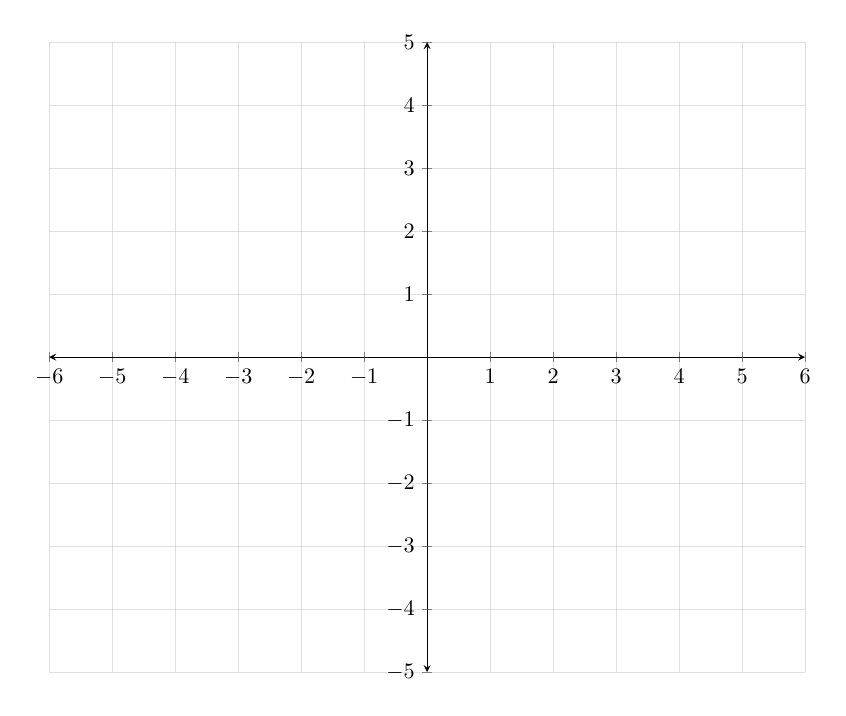
\begin{tikzpicture}[>=stealth, scale=.8]
		\begin{axis}[xmin = -6, xmax=6, ymin=-5, ymax=5, axis x line=middle, axis y line=middle, axis line style=<->, xlabel={}, ylabel={}, grid=both, grid style = {opacity=.5}, clip=false, xtick distance = 1, ytick distance=1, x=1cm, y=1cm]
		\end{axis}
	\end{tikzpicture}
\end{center}
\item Déterminer, par lecture graphique, s'il existe des valeurs $x \in \R$ pour lesquelles $\abs{x} = \dfrac23 x +1$. 
Si oui, combien de telles valeurs existe-t-il ?
\item Justifier, par le calcul, que :
\[ f \Bigpar{ - \dfrac35} = g \Bigpar{- \dfrac35} \et f(3) = g(3) . \]
\end{enumerate}
}{exe:4}{
\begin{enumerate}
\item 
\begin{center}
	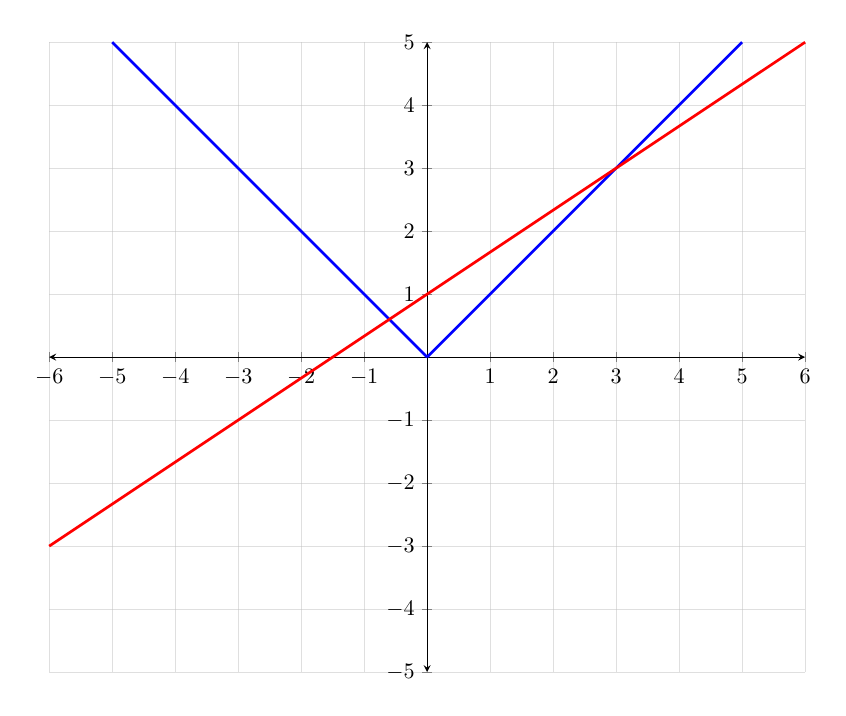
\begin{tikzpicture}[>=stealth, scale=.8]
		\begin{axis}[xmin = -6, xmax=6, ymin=-5, ymax=5, axis x line=middle, axis y line=middle, axis line style=<->, xlabel={}, ylabel={}, grid=both, grid style = {opacity=.5}, clip=false, xtick distance = 1, ytick distance=1, x=1cm, y=1cm]
		\addplot[blue, very thick, domain =0:5, samples=2] {x} ;
		
		\addplot[blue, very thick, domain =-5:0, samples=2] {-x} ;
		\addplot[red, very thick, domain =-6:6, samples=2] (x,{2/3*x+1});
		\end{axis}
	\end{tikzpicture}
\end{center}
\item Il existe deux telles valeurs de $x$, ce sont les points d'intersection des deux courbes.
\item Il suffit de faire les calculs.
\end{enumerate}
}


\exe{}{ (Bonus)
On donne $(1~414)^2=1~999~396$ et $(1~415)^2=2~002~225$. \\
Proposer un encadrement d'amplitude $10^{-3}$ de $\sqrt{2}$.
}{exe:b}{
On remarque $\sqrt{2~000~000} = \sqrt{2} \times 1~000$. Comme $(1~414)^2 < 2~000~000 < (1~415)^2$, en passant à la racine
carrée, on obtient 
\[ 1~414 < \sqrt{2} \times 1~000 < 1~415 \Rightarrow 1,414 < \sqrt{2} < 1,415 . \]
Note : la validité de cet encadrement repose sur le fait que la fonction racine carrée est croissante, donc préserve l'ordre. 
Cette notion n'a pas été abordée, c'est pourquoi aucune justification n'était demandée.
}


%%%%%%%%%%%%

\newpage
\fancyhead[C]{\textbf{Solutions}}
\shipoutAnswer

\end{document}
 